\chapter{Introductie}
\label{ch:introdcution}

\section{Achtergrond en aanleiding}
Rond 2008 begon \&ranj narratieven te verwerken in serious games om op verhalende wijze positieve gedragsverandering, zoals gezonder leven, toe te passen. Door gebruik te maken van de standaardisatie wist het bedrijf op een efficiënte manier meer dan 400 narrative game oplossingen te realiseren op klant specifieke problemen.

De narrative games van \&ranj dienen als een simulatie; een veilige omgeving waarin vooral soft skills beoefend kunnen worden. Soft skills zijn leiderschap, probleemgerichtheid en communicatieve vaardigheden. In het werkveld is er steeds meer vraag naar deze skills\cite{Gibert2017}\cite{Hirsch2017}\cite{Robles2012}. Echter zijn soft skills minder makkelijk te leren en te toetsen op scholen\cite{BishnuMurti2014}. Hiernaast kunnen dergelijke soft skills technische vaardigheden, ook wel hard skills genoemd, bevorderen\cite{Schulz2008}. Met deze games brengt \&ranj lastige onderwerpen ter tafel zoals peace building\footnote{https://ranj.com/projects/corporate/development\#missionzhobia} en discriminatie \footnote{https://ranj.com/projects/education\#fair-play}. Het doel van deze simulaties is dan ook om de speler bewust te maken van de gemaakte keuzes en positieve gedragsverandering te stimuleren.

\begin{wrapfigure}{r}{0.4\textwidth}
    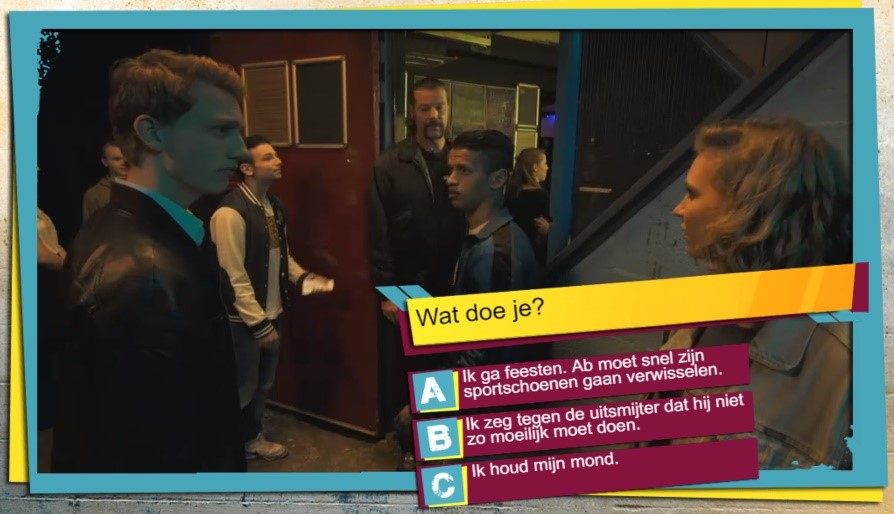
\includegraphics[width=0.38\textwidth]{FairPlayScreen}
    \caption{Een dialoog in de narrative game "Fair Play".}
    \label{fig:fairplayscreen}
    \centering
\end{wrapfigure}

Een narrative game bestaat uit een verhaallijn waarin de speler gesprekken voert met virtuele karakters om het verhaal te vorderen. Dit is goed terug te zien in de game “FairPlay” (\autoref{fig:fairplayscreen}). De games van \&ranj maken gebruik van fotografie, tekst en eventuele video en voice-overs om de speler in het verhaal te plaatsen (\autoref{fig:fairplayscreen}). Deze assets noemen we ook wel game content. Keuzes die de speler maakt hebben invloed op de loop en uitkomst van het verhaal. De speler krijgt directe feedback op zijn of haar gemaakte keuzes. Zo reflecteert het spel op eerder gemaakte keuzes in de vorm van een dialoog of report.

Met nieuwe hedendaagse technologieën wilt \&ranj haar narrative games naar het volgende niveau tillen. Deze toekomstblik noemen ze ‘narrative 2.0’ en staat op de roadmap van \&ranj. Als use case voor narrative 2.0 beschrijft het bedrijf een ‘bad news’ dialoog; een gesprek waarbij de speler slecht nieuws moet brengen. Een voorbeeld van een bad news gesprek is een ‘negatieve’ diagnose die als dokter gegeven moet worden. Deze dialogen willen ze zo realistisch mogelijk maken; succes hangt af van timing en gevoel. Realisme in games wil het bedrijf bereiken door onder andere artificial intelligence (AI) oplossingen toe te passen.

\pagebreak
Om narrative 2.0 te ondersteunen is er vraag naar tooling, externe hulpprogramma(s) die productiviteit bevorderen\cite{Pizzi}, die zal helpen bij het ontwikkelproces van de toekomstige narrative games. Het bedrijf beschikt over twee applicaties waarin narratieven geschreven kunnen worden zonder enige programmeerkennis. Deze applicaties heten de story- en dialog editor en spelen een grote rol in het ontwikkelproces van een narrative game. In deze bewerkers wordt content voor de game gespecificeerd die later afgespeeld zal worden door de game engine. Ze bestaan uit een interface waarin content types in nodes worden gerepresenteerd. Een content type is een datastructuur met een betekenis in de game. Het content type ‘ImageContent’ zou bijvoorbeeld als doel hebben om een afbeelding tonen. Tenslotte verbinden edges de content met elkaar (\autoref{fig:visualscriptingineditor}).

Deze story- en dialog editor heeft het bedrijf in 2008 opgezet met behulp van de Apache Flex SDK en ActionScript3. Over de jaren heen zijn de verwachtingen van de bewerkers veranderd, maar ze zijn niet uitgebreid omdat de achterliggende softwarearchitectuur niet houdbaar en flexibel is. Dit zorgt voor problemen bij het ontwikkelproces van zowel huidige als toekomstige narrative games zoals de ‘bad news’ game. \&ranj wilt inzicht krijgen in wat er nodig is om een nieuwe editor op te zetten die oplossingen biedt op de huidige problemen.

\begin{figure}[htb]
    \centering
    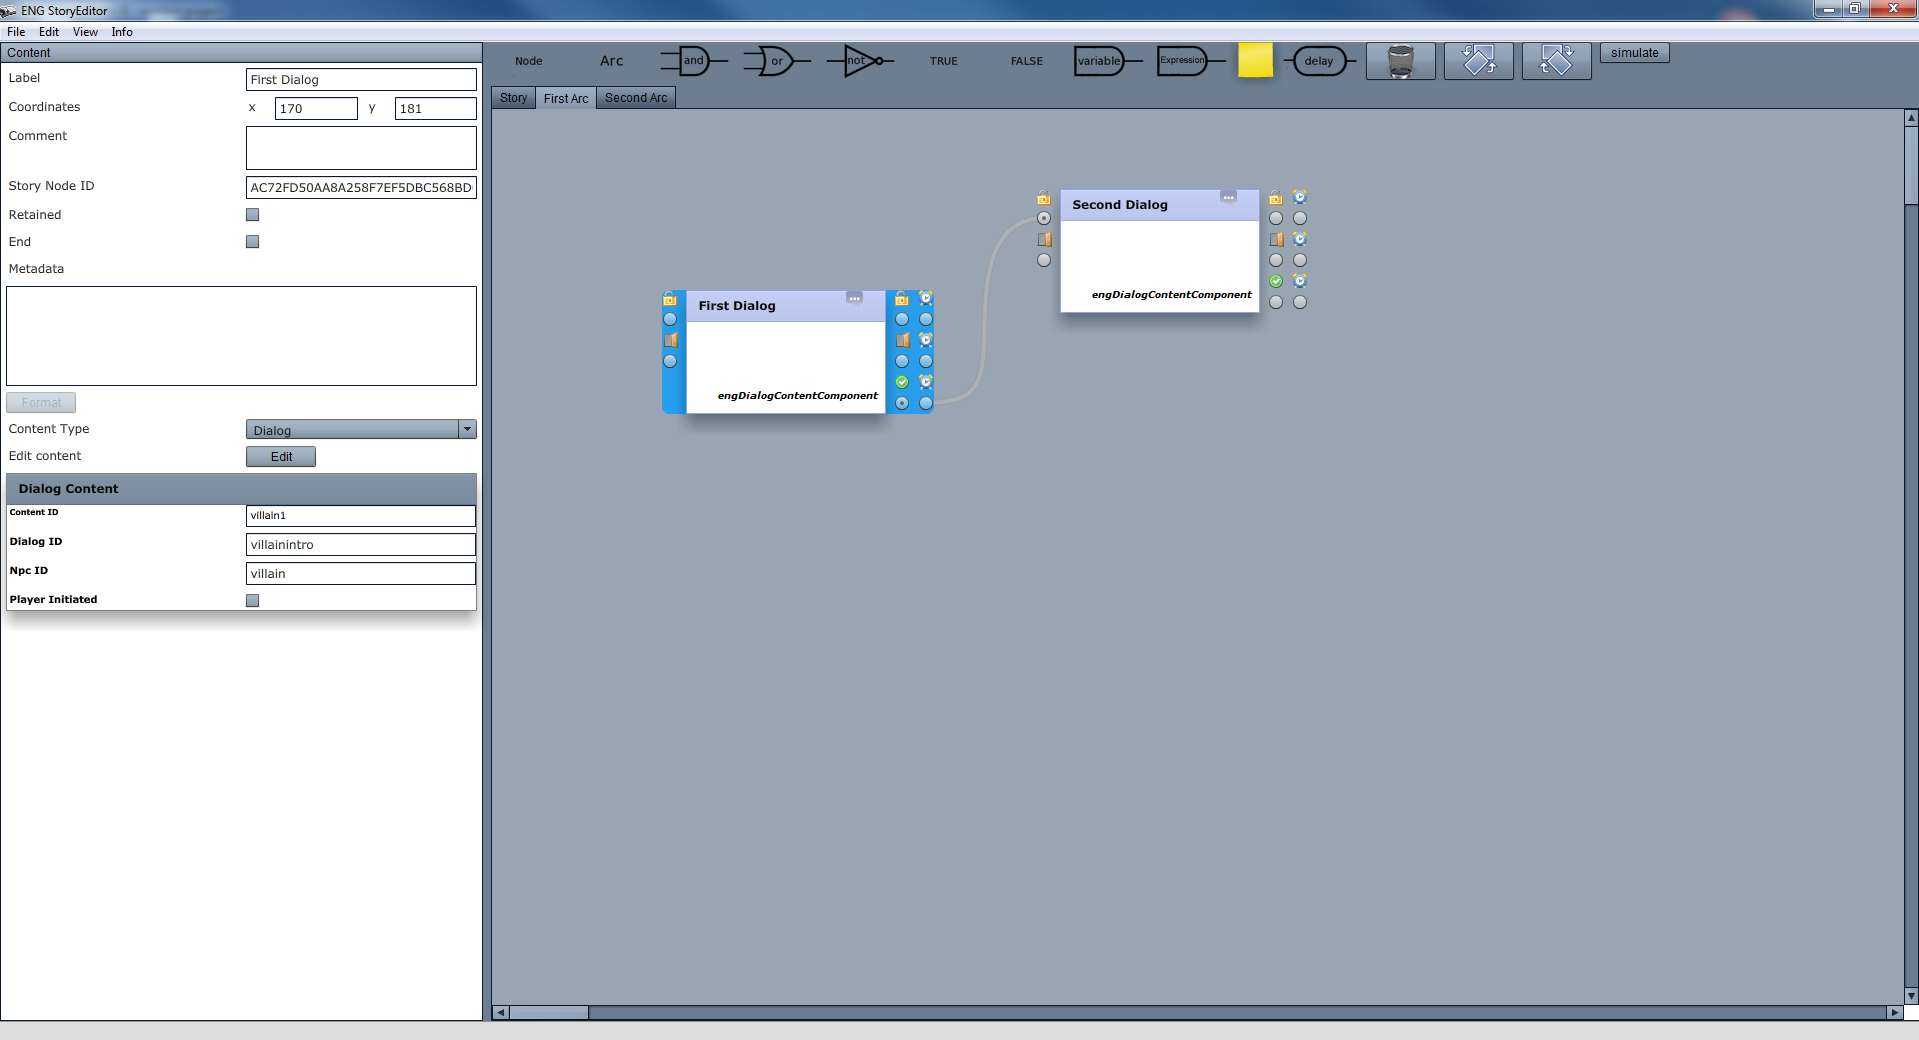
\includegraphics[width=0.92\textwidth]{VisualScriptingInEditor}
    \caption{Visual scripting in de Story Editor.}
    \label{fig:visualscriptingineditor}
\end{figure}

\pagebreak
\section{Probleemstelling}
De story- en dialog editor zijn opgezet om medewerkers zonder programmeerkennis game content zelfstandig te laten bewerken. Deze tooling wordt gebruikt in alle narrative game projecten en is essentieel voor het ontwikkelproces en productiviteit. Hiernaast bevordert het itereren over game content en maakt deze inzichtelijk door de game content te visualiseren. Hierbij speelt flexibiliteit een grote rol. De editors moeten flexibel genoeg zijn om bruikbaar te zijn voor verschillende narrative game projecten.

Het bedrijf werkt toe naar nieuwe tooling en wilt inzicht verkrijgen in het opzetten van flexibele oplossingen. Dit leidt dan ook tot de centrale onderzoeksvraag: 

\begin{quote} 
    \centering
    \large
    \textit{
        "Hoe kan er een flexibele tool worden opgezet voor het vertellen van diverse digitale interactieve verhalen?"
    }
\end{quote}

\subsection{Technologieën}
De levensduur van een applicatie hangt onder andere af van de technologieën waarop deze gebouwd is. Het opzetten van een tool kan veel tijd en werk kosten. Om profijt te halen uit deze investering is het van belang dat de tool voor een langere periode inzetbaar is. De onderliggende bouwblokken van de applicatie moet toekomstgericht zijn. Een grote community en sponsoren rondom een technologie bieden meer zekerheid dat de technologie langer zal blijven bestaan en onderhouden zal worden. Daarnaast kunnen eventuele toekomstwensen van het bedrijf invloed hebben op technologische keuzes. Het is essentieel om een toekomstgerichte selectie te maken uit bestaande technologieën waarop de tool gebouwd zal worden.

Het huidige gebruikte platform, Apache Flex, heeft weinig libraries die gebruikt kunnen worden voor de interface van de editors. Libraries zijn collecties aan code en configuraties die gebruikt kunnen worden in andere applicaties. Meestal richten ze zich op een veelvoorkomend probleem, zodat programmeurs niet telkens het wiel opnieuw uit hoeven te vinden. De libraries die beschikbaar zijn voor Apache Flex, zoals ‘Flex Wires’ die de verbindingen tussen nodes mogelijk maakt, hebben weinig functionaliteit en bevatten bugs. \&ranj wilt naar een platform met een grotere community en meer flexibiliteit in frameworks en libraries, zodat het wiel niet telkens opnieuw uitgevonden hoeft te worden.

Voor \&ranj is het ultieme einddoel om een webapplicatie te realiseren waarin meerdere personen tegelijk aan een narratief kunnen werken. Collaborative editing, het ondersteunen van aanpassingen door meerdere personen tegelijk, kan het onder andere makkelijker maken om samen met klanten te werken.

\subsection{Diversiteit in game content}
Narrative games zijn games gedreven door een verhaal. Tekstuele inhoud wordt verworven met visuals, media en spelelementen. Deze inhoud in zijn geheel wordt ook wel game content genoemd en verschilt per game. Narrative games kunnen verschillende spelelementen bevatten, waaronder quizzen en het verzamelen van data door het ontvangen van sms’jes/ e-mails. Games bevatten slechts een selectie aan spelelementen waardoor de game content van de ene game sterk kan verschillen met die van een andere game.

Uit eerdere projecten die verschillen in game content blijkt dat de huidige editors niet flexibel genoeg zijn. Het probleem ligt vooral aan de diversiteit in game content tussen projecten. Echter is dit wel een eis sinds \&ranj voor verschillende klanten werkt waarvan ieder een eigen beroepenveld heeft. Dit dwingt diversiteit in game content af.

In de game content speelt semantiek een grote rol. De interpretatie van een content type hangt af van haar semantische eigenschappen. In de huidige editors hebben content types een statische definitie. Om nieuwe content types toe te voegen moeten de content types gedefinieerd worden in de broncode; content types zijn hard gebakken in de editors. Het opzetten, uitbreiden, compileren en deployen van de editors is een langdurig proces dat met de hand uitgevoerd moet worden. Voor ieder project moeten er nieuwe editors met de benodigde content types worden gebouwd. Hierbij moet er ook nog eens op gelet worden dat oudere content types functioneel blijven, zodat de editors de data van oudere narrative games nog kunnen uitlezen. Dit maakt het erg lastig om de huidige story- en dialog editor in te zetten voor verschillende projecten vanwege de tijd en dus geld die het kost om content types toe te voegen. Vaak wordt dit ondanks de kosten wel gedaan wat resulteert in een uitbreidende selectie aan content types. Echter zijn deze content types meestal zo project specifiek dat ze niet in meer dan één project gebruikt worden. Dit resulteert in een onoverzichtelijke editor, omdat de niet gebruikte content types wel in de editor zitten.

\subsection{Het ondersteunen van meerdere formalismen}
In de huidige editors bestaat er een nauwe koppeling tussen de visual scripting interface en het achterliggende formalisme. Dit maakt het lastig om van formalisme te veranderen, laat staan nieuwe formalisme te ondersteunen. Deze beperking verlaagd de flexibiliteit en inzetbaarheid van de editors. In de roadmap van het bedrijf wordt beschreven hoe \&ranj een ‘smart follower’ wilt zijn onder andere op het gebied van artificial intelligence (AI). Er gebeurt erg veel op het gebied van AI en \&ranj ziet mogelijkheden om deze nieuwe technologie toe te passen in toekomstige games. Door op de hoogte te blijven van AI kan het bedrijf nieuwe aantrekkelijke oplossingen verwerken in hun games en deze verkopen aan de klant. Met de huidige story- en dialog editor is het vrijwel onmogelijk om gebruik te maken van AI. Het achterliggende formalisme biedt alleen de mogelijkheid om content types aan elkaar te verbinden en zo een graph te vormen. Om AI toe te passen in narrative games moet er gebruik gemaakt worden van formalismen die dit ondersteunen. In tegenstelling tot het huidige formalisme waarin opeenvolgende instructies gedefinieerd worden bieden behaviour trees een meer AI georiënteerde oplossing\cite{Pizzi}\cite{Lim2010}.

\subsection{Overkoepelende projectstructuur}
Hoewel de dialog- en story editor het narratief ordent en aan elkaar verbindt beheert zij de bijbehorende game content niet; er is geen sprake van een overkoepelde projectstructuur. Een voorbeeld hiervan is hoe de huidige editors om gaan assets, bestanden die gebruikt worden in de game. Er moet handmatig een manifest worden bijgehouden waarin assets een sleutel (id) en semantiek toegekend krijgen (zie \autoref{fig:gamecontentmanifest}). Deze sleutel wordt gebruikt in de huidige editors om te kunnen refereren naar assets, zoals geluid, afbeeldingen en videos. Zo refereert het content type ‘image content’ naar een asset via een sleutel. Deze asset zou een afbeelding moeten zijn, maar er bestaat geen zekerheid over dat de asset een afbeelding is of überhaubt bestaat. Dit zorgt voor een zwakke link tussen de editors en game content, wat het erg gevoelig maakt voor (menselijke)fouten. Zo hoeft er maar één typefout gemaakt of het pad aangepast te worden om de referentie naar de game content te verliezen.

\begin{figure}[htb]
    \centering
    \lstset{language=JSON}
    \begin{lstlisting}
    {
        "scenario_test": [{
            "id": "story_scenario_test",
            "type": "json",
            "src": "assets/scenarios/scenario_test/story.json"
        }],
        "sounds": [{
            "id": "backgroundmusic",
            "type": "sound",
            "src": "assets/sounds/backgroundmusic.mp3"
        }]
    }
    \end{lstlisting}
    \caption{Game content manifest.}
    \label{fig:gamecontentmanifest}
\end{figure}

\pagebreak
\section{Doelstelling}
\subsection{Vanuit \&ranj}
Het bedrijf hoopt in 2019 nieuwe editor(s) op te zetten die het ontwikkelproces van narrative games zullen ondersteunen. Om de diversiteit in klanten en de toekomstplannen van de editors te ondersteunen moeten de nieuwe editor(s) flexibel opgezet zijn, zodat het op maat maken van de games mogelijk is. Zo moet de nieuwe editor kunnen omgaan met de diversiteit in game content, een deel uit maken van een overkoepelende projectstructuur en het achterliggende formalisme scheiden van de user interface.

\subsection{Uit persoonlijk interesse}
\begin{wrapfigure}{r}{0.4\textwidth}
    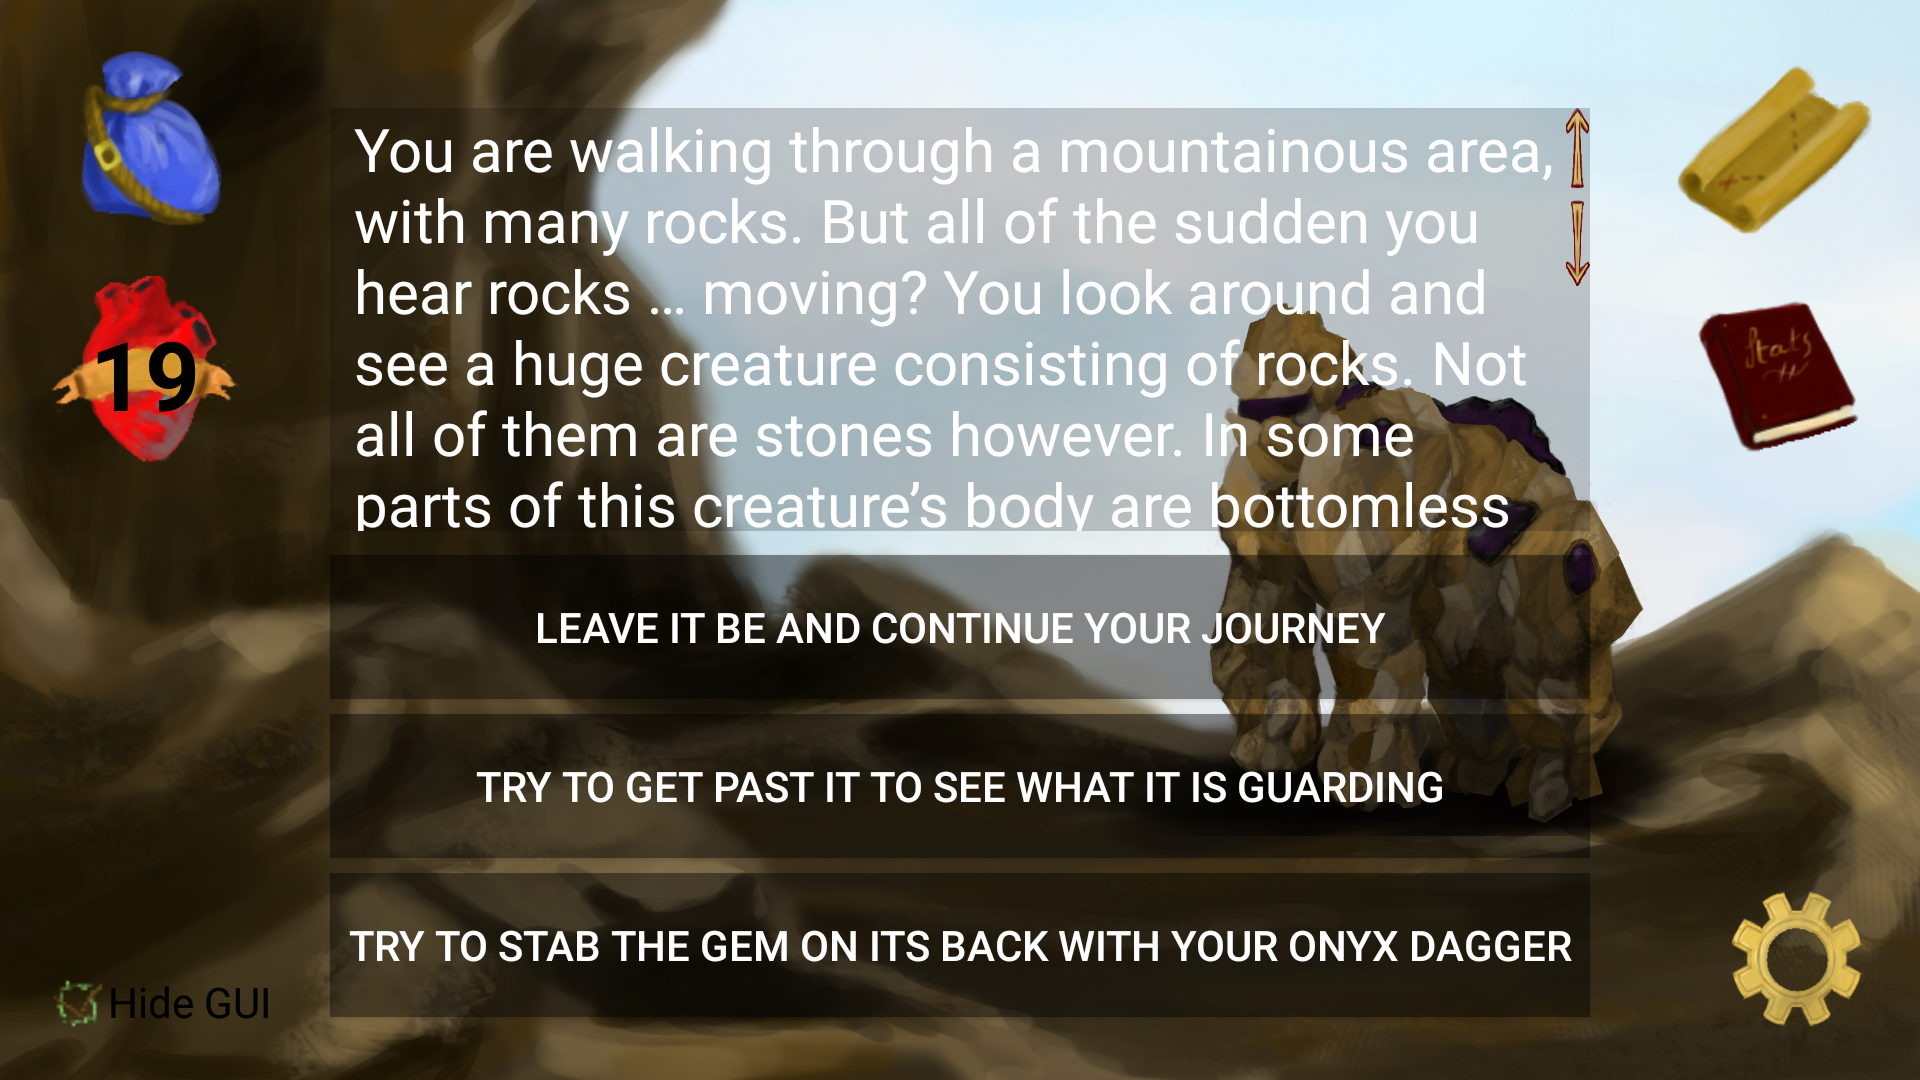
\includegraphics[width=0.38\textwidth]{ReignOfDwarves}
    \caption{Een screenshot van het zelfstandige narrative game project.}
    \label{fig:reignofdwarves}
    \centering
\end{wrapfigure}
Mijn eerste aanraking met een narrative game was een zelfstandig project drie jaar geleden (zie \autoref{fig:reignofdwarves}). Er was een duidelijke behoefte naar tooling om het verhaal in te schrijven. Het makkelijk kunnen aanpassen van het verhaal was een probleem, omdat er geen externe tooling voor bestond die goed aansloot bij de wensen van het project destijds. Hoewel het een erg leuk project was om naast mijn studie op te pakken, bracht het veel werk met zich mee waardoor het nooit gelukt is om het project af te ronden. Dit onderzoek kan inzicht bieden in hoe dit beter aangepakt had kunnen worden.

\subsection{Vanuit school}
Het onderzoek moet gedocumenteerd worden in de vorm van een scriptie. Deze scriptie moet voldoen aan de beoordelingscriteria die vooraf opgesteld zijn. Er moet tijdens het onderzoek voldaan worden aan 4 competenties: beheren, analyseren, adviseren en ontwerpen. Tenslotte moet er sprake zijn van een professionele houding en adequate communicatie met de stakeholders. De beoordeling volgt uit de scriptie en eindpresentatie.


\section{Onderzoeksvragen}
\subsection{Hoofdvraag}
Vanuit het probleem is de volgende centrale onderzoeksvraag opgesteld:
\begin{quote} 
    \centering
    \large
    \textit{
        "Hoe kan er een flexibele tool worden opgezet voor het vertellen van diverse digitale interactieve verhalen?"
    }
\end{quote}

\subsection{Deelvragen}
Om de centrale onderzoeksvraag te kunnen beantwoorden zijn de volgende deelvragen opgesteld:
\begin{enumerate}
    \item Hoe kan er een ‘technology stack’ opgezet worden die een flexibele basis biedt voor een editor waarmee diverse digitale interactieve verhalen verteld kunnen worden?
    \item Hoe kan diverse game content ondersteund worden?
    \item Hoe kan de architectuur achter de editor zo worden opgezet dat er in latere stadia nieuwe narratieve formalismen makkelijk doorgevoerd kunnen worden?
    \item Hoe kan game content in een overkoepelende projectstructuur verbonden en geordend worden?
\end{enumerate}
Hierbij is de eerste deelvraag een vereisten voor het opzetten van de editor. De tweede, derde en vierde deelvragen tackelen pijnpunten die voorkomen in de huidige editor en zullen de flexibiliteit van de nieuwe editor bevorderen. De gespecificeerde deelvragen bouwen voort op elkaar; het resultaat van een deelvraag kan de uitwerking van opvolgende deelvragen beïnvloeden. Zo heeft het resultaat van de eerste deelvraag invloed op deelvragen 2, 3 en 4. Tenslotte komt er een vervolgonderzoeksvraag voort uit de tweede deelvraag die beantwoord zal worden met de vierde deelvraag.

\section{Scope}
Het onderzoek vindt plaats over een tijdsduur van 20 weken. Omdat er gewerkt wordt met een tijdslimiet is het belangrijk om een scope vast te leggen. Naast dat deze afbakening overzicht en focus biedt voorkomt deze misverstanden tussen de betrokken partijen.

\noindent Dit onderzoek omvangt:
\begin{itemize}
    \item Het doorspitten van de broncode achter de huidige editors.
    \item Eventuele prototypes om standpunten te onderbouwen.
    \item Advies op het gebied van ontwikkelplatformen, libraries en architectuur.
    \item Het in kaart brengen van de huidig gebruikte technologieën.
    \item Een scriptie schrijven met daarin adviezen en conclusies over het desbetreffende onderwerp.
\end{itemize}

\noindent Er zal geen aandacht besteed worden aan:
\begin{itemize}
    \item Het ontwikkelen van een productie klare editor die direct inzetbaar is voor toekomstige narrative game projecten.
    \item Een narrative game ontwikkelen met de eventuele gemaakte prototypes.
    \item Verdieping in klant co-creatie.
    \item Onderzoek naar ‘collaborative editing’.
    \item De deployment pipeline van de editors.
    \item Optimalisatie van de editors.
    \item Het dataformaat waarmee de editors communiceren met de game engine.
\end{itemize}

\section{Structuur}
Deze paragraaf geeft inzicht in de komende hoofdstukken van de scriptie en dient als een kapstok voor de lezer. Zo wordt er bij ieder hoofdstuk beschreven wat de lezer kan verwachten.

\begin{description}
    \item[Hoofdstuk 2] omschrijft welke methodes er gebruikt zijn om tot de behaalde resultaten te komen.
    \item[Hoofdstuk 3] geeft context aan het onderzoek en plaats deze in een groter plaatje.
    \item[Hoofdstuk 4] betreft de onderliggende bouwblokken waarop de huidige applicatie gebouwd is en waarop de nieuwe applicatie gebouwd zal worden; de ‘technology stack‘. Het belang van een goedpassende tech stack komt ter sprake en er worden adviezen gedaan over benodigde veranderingen binnen de stack die aansluiten op het toekomstbeeld bij de editors.
    \item[Hoofdstuk 5] beschrijft hoe er onderscheid wordt gemaakt tussen game content. Hiernaast gaat dit hoofdstuk in op de diversiteit in game content en hoe deze ondersteund kan worden.  
    \item[Hoofdstuk 6] betreft de rol van formalisme binnen interactive story telling, de formalismen die gebruikt worden in de huidige editors en het leggen van een scheiding tussen de editors en achterliggende formalisme.
    \item[Hoofdstuk 7] gaat in op de behoefte aan een overkoepelende projectstructuur en eventuele stappen die gemaakt kunnen worden.
    \item[Hoofdstuk 8] beschrijft de eindconclusie van het onderzoek.
    \item[Hoofdstuk 9] geeft inzicht in de adviezen die voort zijn gekomen uit het onderzoek. Hiernaast komen ook eventuele aandachtspunten of vervolgonderzoek ter sprake.
    \item[Hoofdstuk 10] omvat een reflectie op de afstudeerstage het onderzoek.
    \item[Hoofdstuk 11] bevat een lijst met begrippen en verwijzingen naar waar het begrip staat uitgelegd.
\end{description}